\documentclass[12pt,letterpaper]{article}

\usepackage{amsmath}
\usepackage{fontspec}
\setromanfont[Ligatures=TeX]{TeX Gyre Pagella}
\usepackage{unicode-math}
\setmathfont{TeX Gyre Pagella Math}
\usepackage[title]{appendix}
\usepackage[margin=1.0in]{geometry}
\usepackage[figuresleft]{rotating}
\usepackage[longnamesfirst]{natbib}
\usepackage{dcolumn}
\usepackage{booktabs}
\usepackage{multirow}
\usepackage[flushleft]{threeparttable}
\usepackage{setspace}
\usepackage[justification=centering,skip=2pt]{caption}
\usepackage[font=scriptsize]{subfig}
\usepackage[xetex,colorlinks=true,linkcolor=black,citecolor=black,urlcolor=black]{hyperref}
\usepackage{adjustbox}
\usepackage{xfrac}
\usepackage{placeins}

\newcommand{\mco}[1]{\multicolumn{1}{c}{#1}}
\newcommand{\mct}[1]{\multicolumn{2}{c}{#1}}
\newcommand{\mcth}[1]{\multicolumn{3}{c}{#1}}
\newcommand{\X}{$\times$ }
\newcommand{\hs}{\hspace{15pt}}

\renewcommand\floatpagefraction{.9}
\renewcommand\topfraction{.9}
\renewcommand\bottomfraction{.9}
\renewcommand\textfraction{.1}
\setcounter{totalnumber}{50}
\setcounter{topnumber}{50}
\setcounter{bottomnumber}{50}


%------------------------------------------------------------------------


\title{Birth Spacing and Fertility in the Presence of Son Preference and Sex-Selective Abortions:
India's Experience Over Four Decades%
\protect\thanks{%
I am grateful to Andrew Foster and Darryl Holman for discussions about the method.
I owe thanks to Monica Das Gupta, Shelly Lundberg, Daniel Rees, David Ribar, 
Hendrik Wolff, three anonymous reviewers, and seminar participants at University of 
Copenhagen, University of Michigan, University of Washington, University of Aarhus, the 
Fourth Annual Conference on Population, Reproductive Health, 
and Economic Development, and the Economic Demography Workshop for helpful 
suggestions and comments.
I would also like to thank Nalina Varanasi for research assistance.
Support for development of the method from the University of Washington Royalty 
Research Fund and the Development Research Group of the World Bank is gratefully 
acknowledged.
The views and findings expressed here are those of the author and
should not be attributed to the World Bank or any of its member countries.
Partial support for this research came from a Eunice Kennedy Shriver National
Institute of Child Health and Human Development research infrastructure grant,
5R24HD042828, to the Center for Studies in Demography and Ecology at the
University of Washington.
Text and code for this paper are available at 
\href{https://github.com/cportner/sexSelectionSpacing}{\texttt{https://github.com/cportner/sexSelectionSpacing}}.
}
}

\author{Claus C P\"ortner\\
    Department of Economics\\
    Albers School of Business and Economics\\
    Seattle University, P.O. Box 222000\\
    Seattle, WA 98122\\
    \href{mailto:cportner@seattleu.edu}{\texttt{cportner@seattleu.edu}}\\
    \href{http://www.clausportner.com}{\texttt{www.clausportner.com}}\\
    \& \\
    Center for Studies in Demography and Ecology \\
    University of Washington\\ \vspace{2cm}
    }

\date{May 2021}


%------------------------------------------------------------------------


\begin{document}
\graphicspath{{./figures/}}
\DeclareGraphicsExtensions{.eps,.jpg,.pdf,.mps,.png}

\setcounter{page}{-1}
\maketitle
\thispagestyle{empty}

\newpage
\thispagestyle{empty}
\doublespacing


\newpage


%------------------------------------------------------------------------


\begin{figure*}[htpb]
\centering
    \begin{minipage}{0.49\textwidth}
        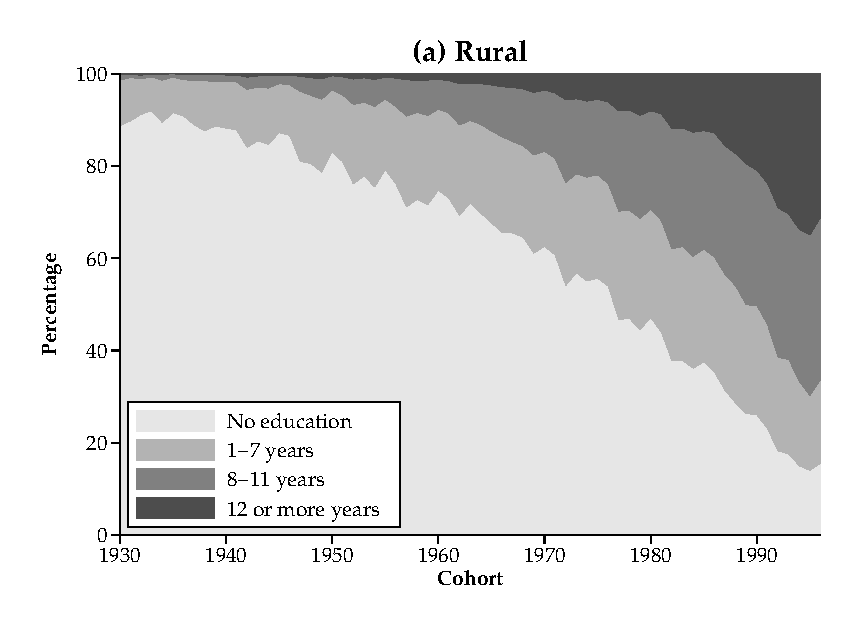
\includegraphics[width=\textwidth]{educ_over_time_rural}
    \end{minipage}
    \begin{minipage}{0.49\textwidth}
        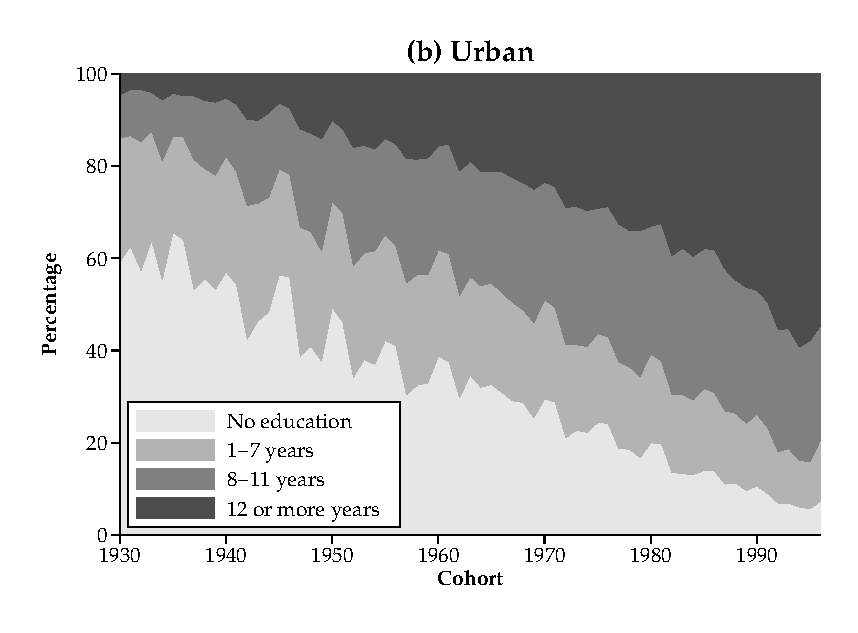
\includegraphics[width=\textwidth]{educ_over_time_urban} 
    \end{minipage}
% \caption{Distribution of education by cohort for women 20 years or older
% using the four rounds of the NFHS}
% \label{fig:education_over_time}
\end{figure*}


\captionsetup[figure]{skip = -16pt}

\begin{figure*}
\centering
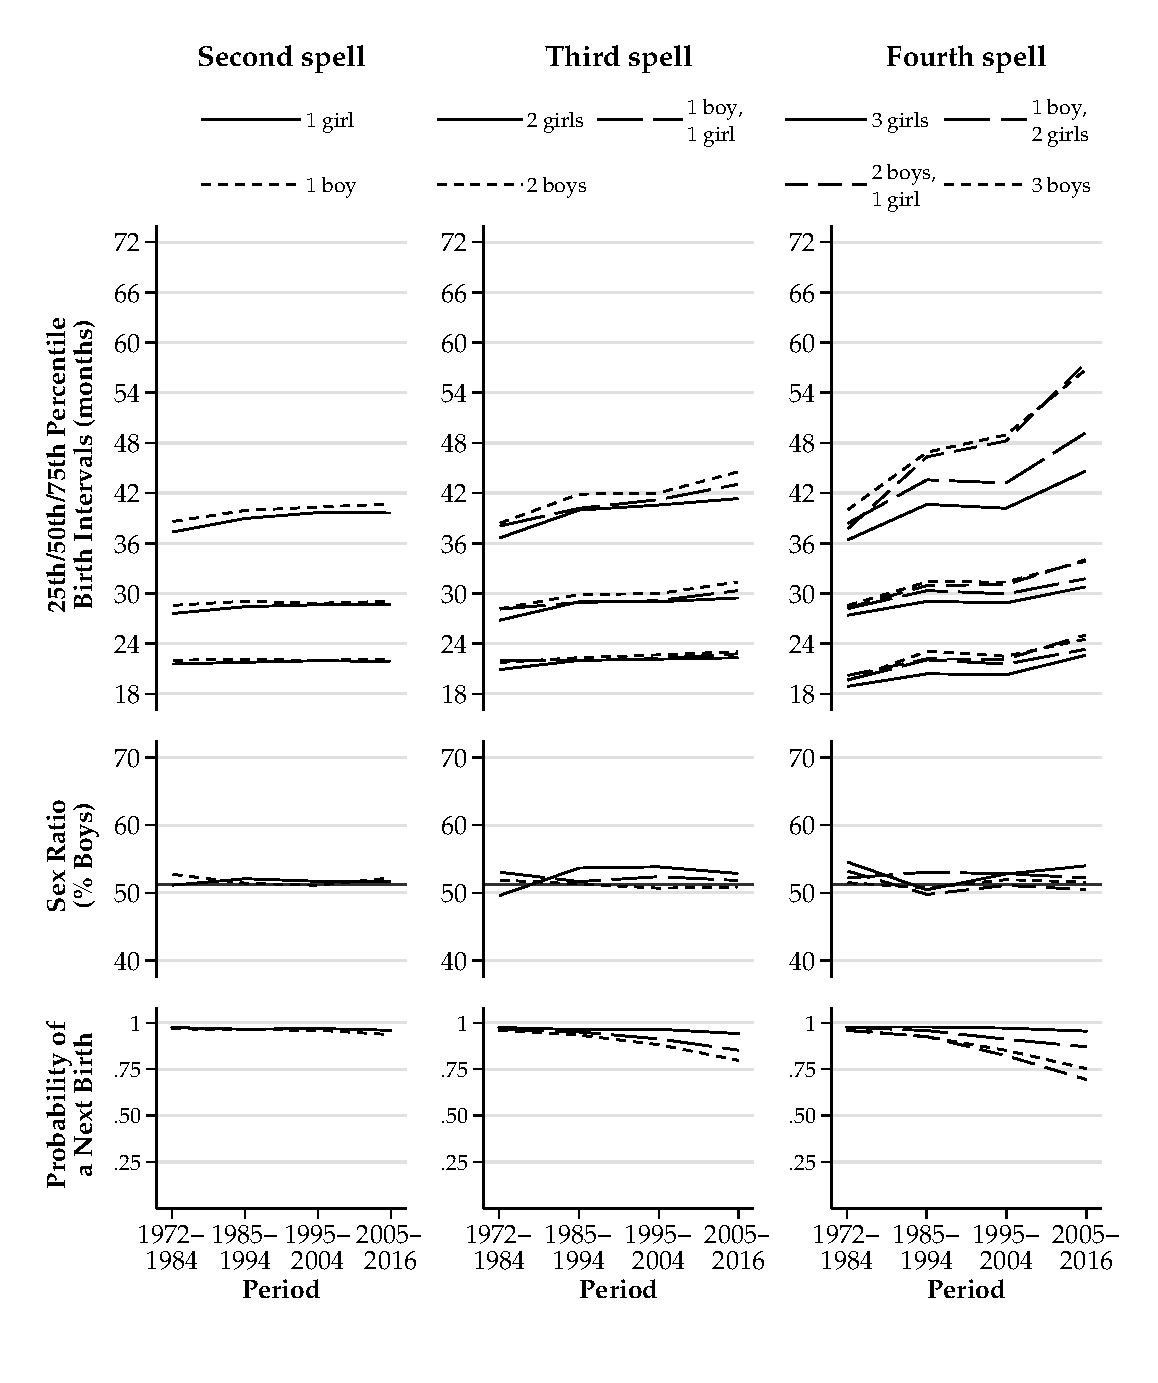
\includegraphics[width=\textwidth,height=\textheight,keepaspectratio=true]{bs_low_rural}
% \caption{Percentile birth interval durations, sex ratios, and parity progression  
% for rural women with no education by spell, sex composition, and period}
% \label{fig:spacing_low_rural}
\end{figure*}

\begin{figure*}
\centering
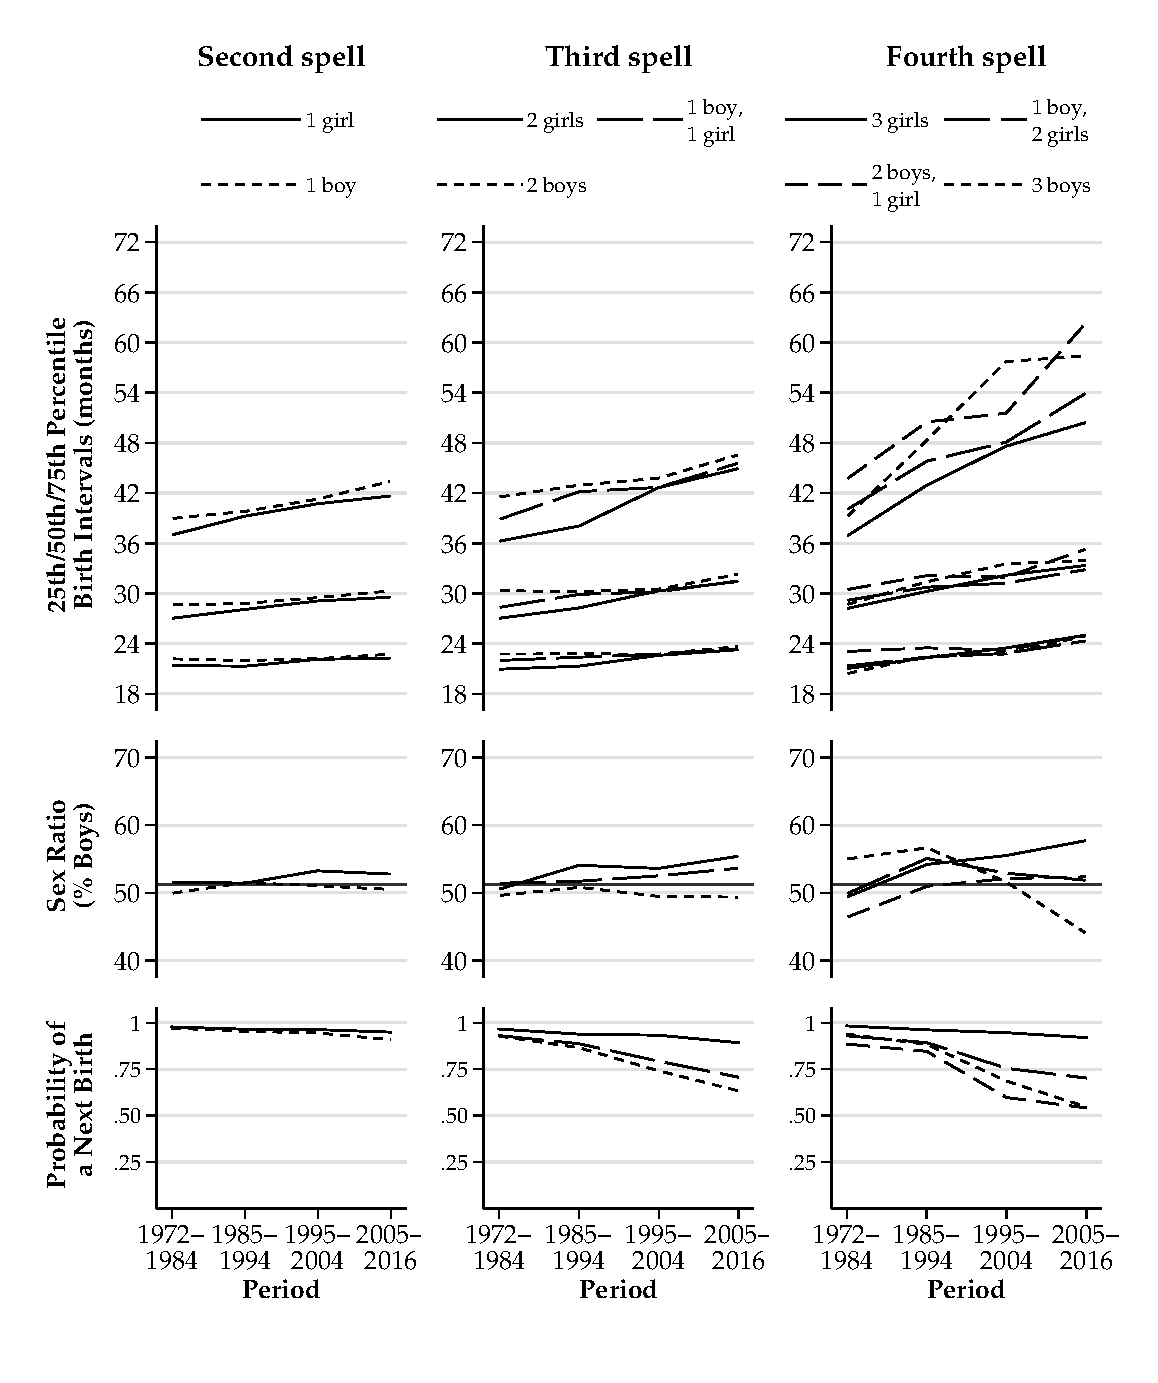
\includegraphics[width=\textwidth,height=\textheight,keepaspectratio=true]{bs_med_rural}
% \caption{Percentile birth interval durations, sex ratios, and parity progression  
% for rural women with 1--7 years of education by spell, sex composition, and period}
% \label{fig:spacing_med_rural}
\end{figure*}

\begin{figure*}
\centering
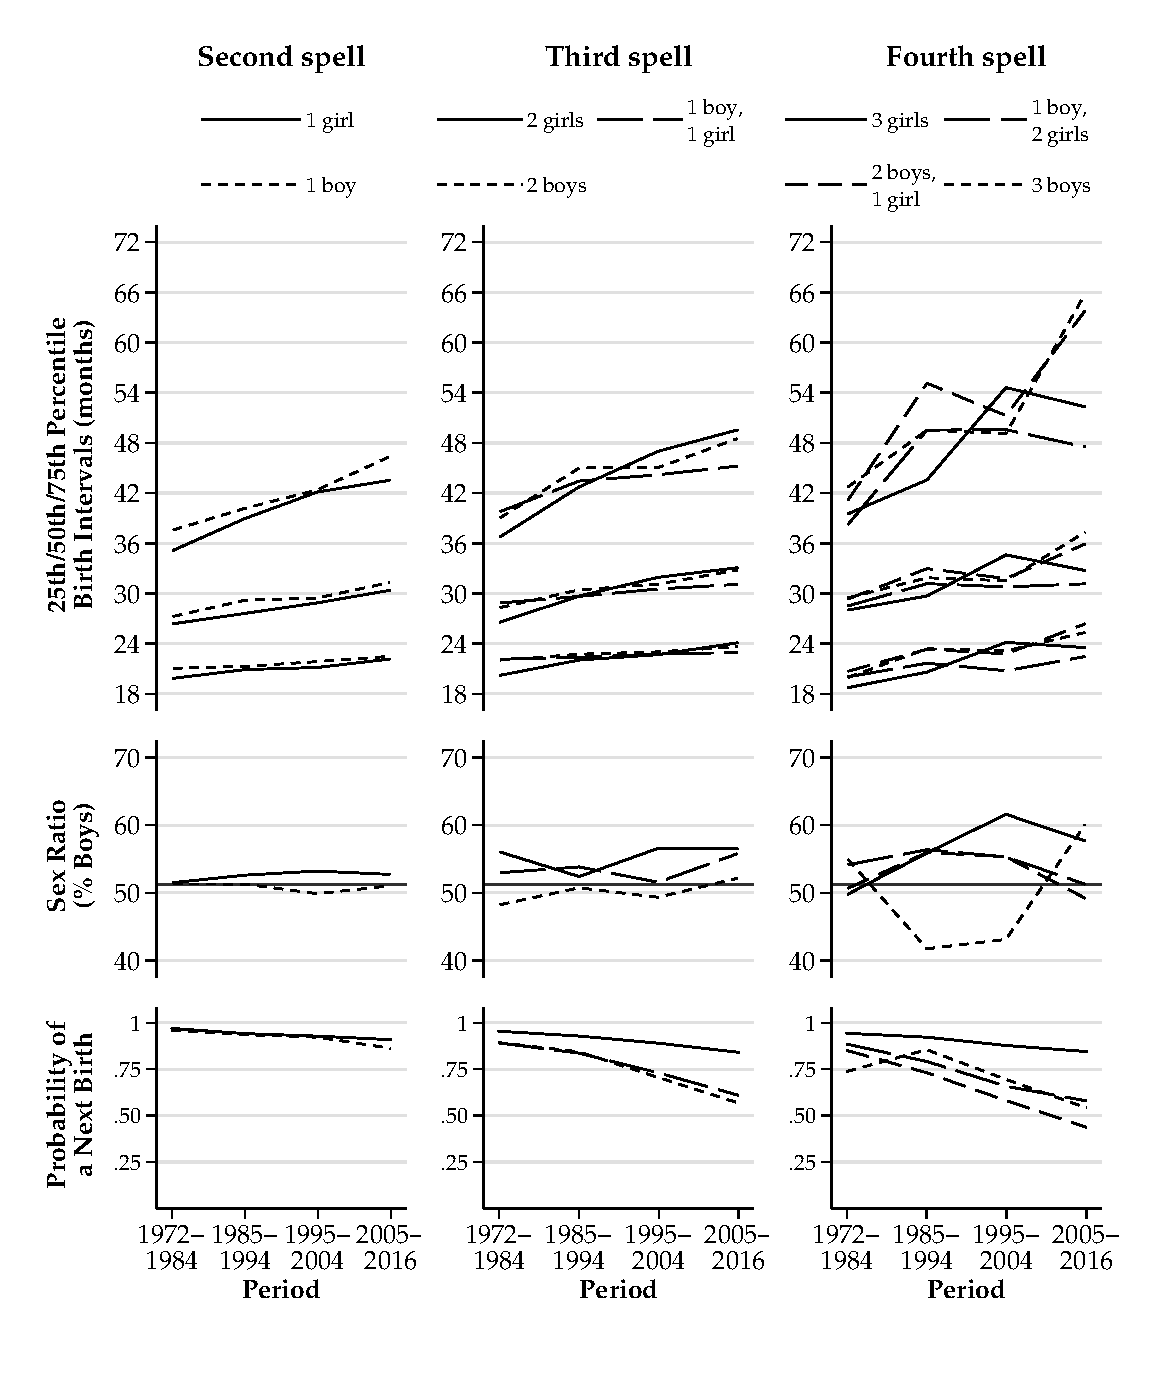
\includegraphics[width=\textwidth,height=\textheight,keepaspectratio=true]{bs_med_urban}
% \caption{Percentile birth interval durations, sex ratios, and parity progression  
% for urban women with 1--7 years of education by spell, sex composition, and period}
% \label{fig:spacing_med_urban}
\end{figure*}

\begin{figure*}
\centering
% 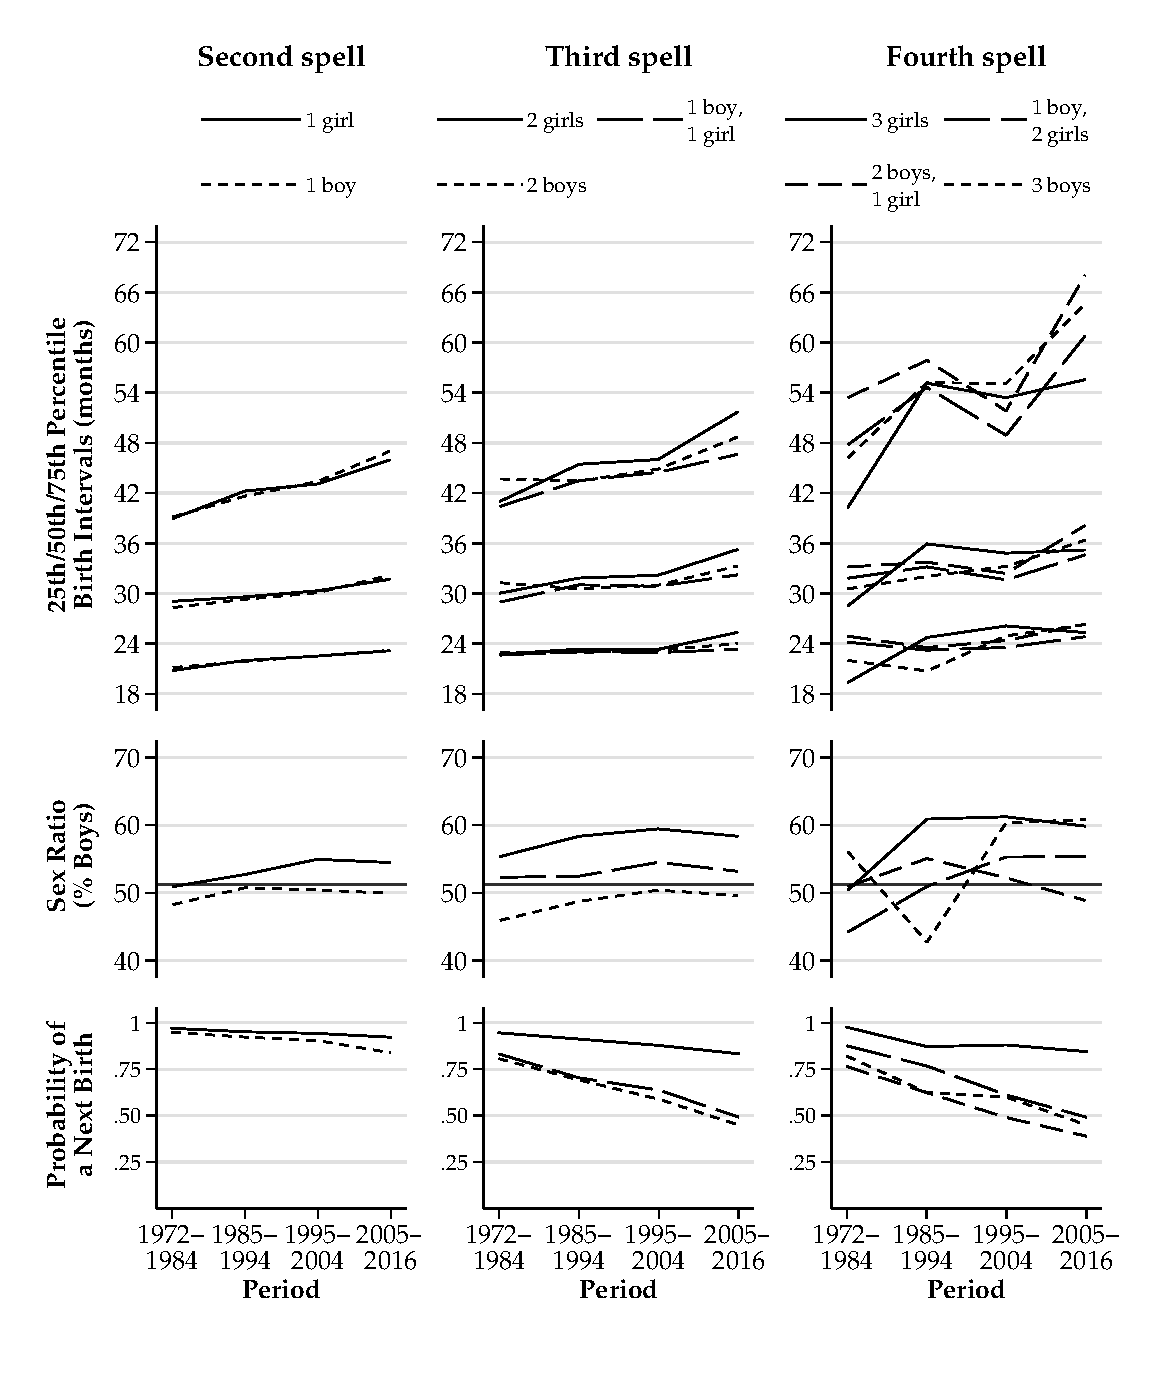
\includegraphics[width=\textwidth,height=\textheight,keepaspectratio=true]{bs_high_rural}
% \caption{Percentile birth interval durations, sex ratios, and parity progression  
% for rural women with 8--11 years of education by spell, sex composition, and period}
% \label{fig:spacing_high_rural}
\end{figure*}

\begin{figure*}
\centering
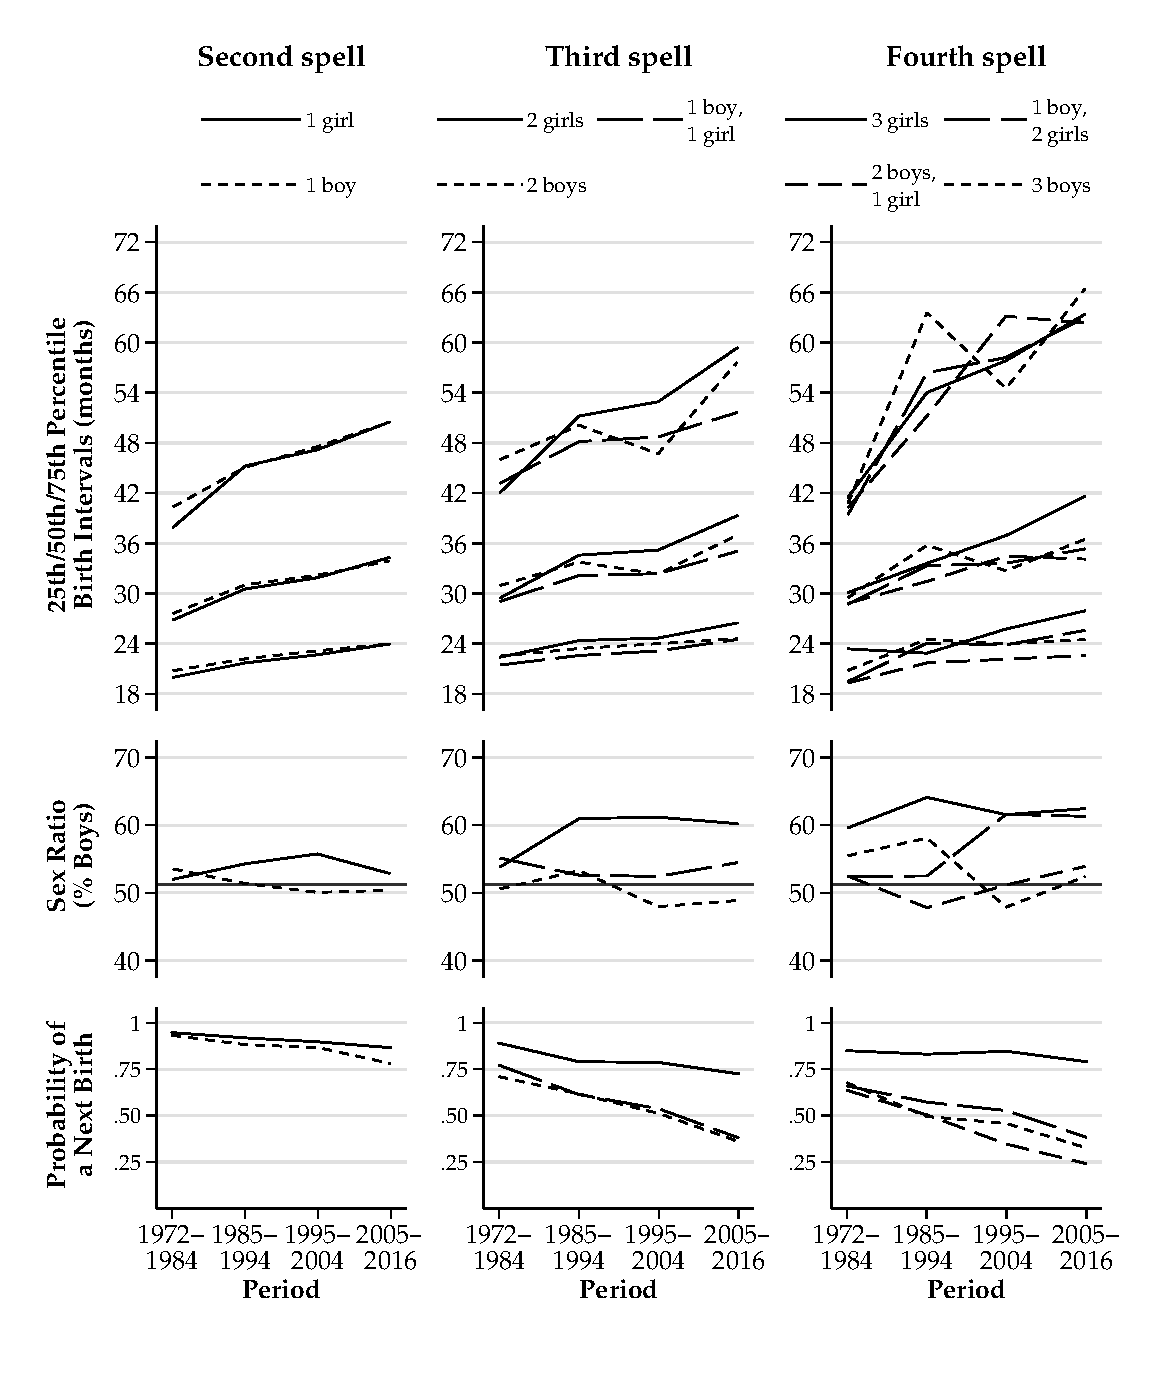
\includegraphics[width=\textwidth,height=\textheight,keepaspectratio=true]{bs_high_urban}
% \caption{Percentile birth interval durations, sex ratios, and parity progression  
% for urban women with 8--11 years of education by spell, sex composition, and period}
% \label{fig:spacing_high_urban}
\end{figure*}

\begin{figure*}
\centering
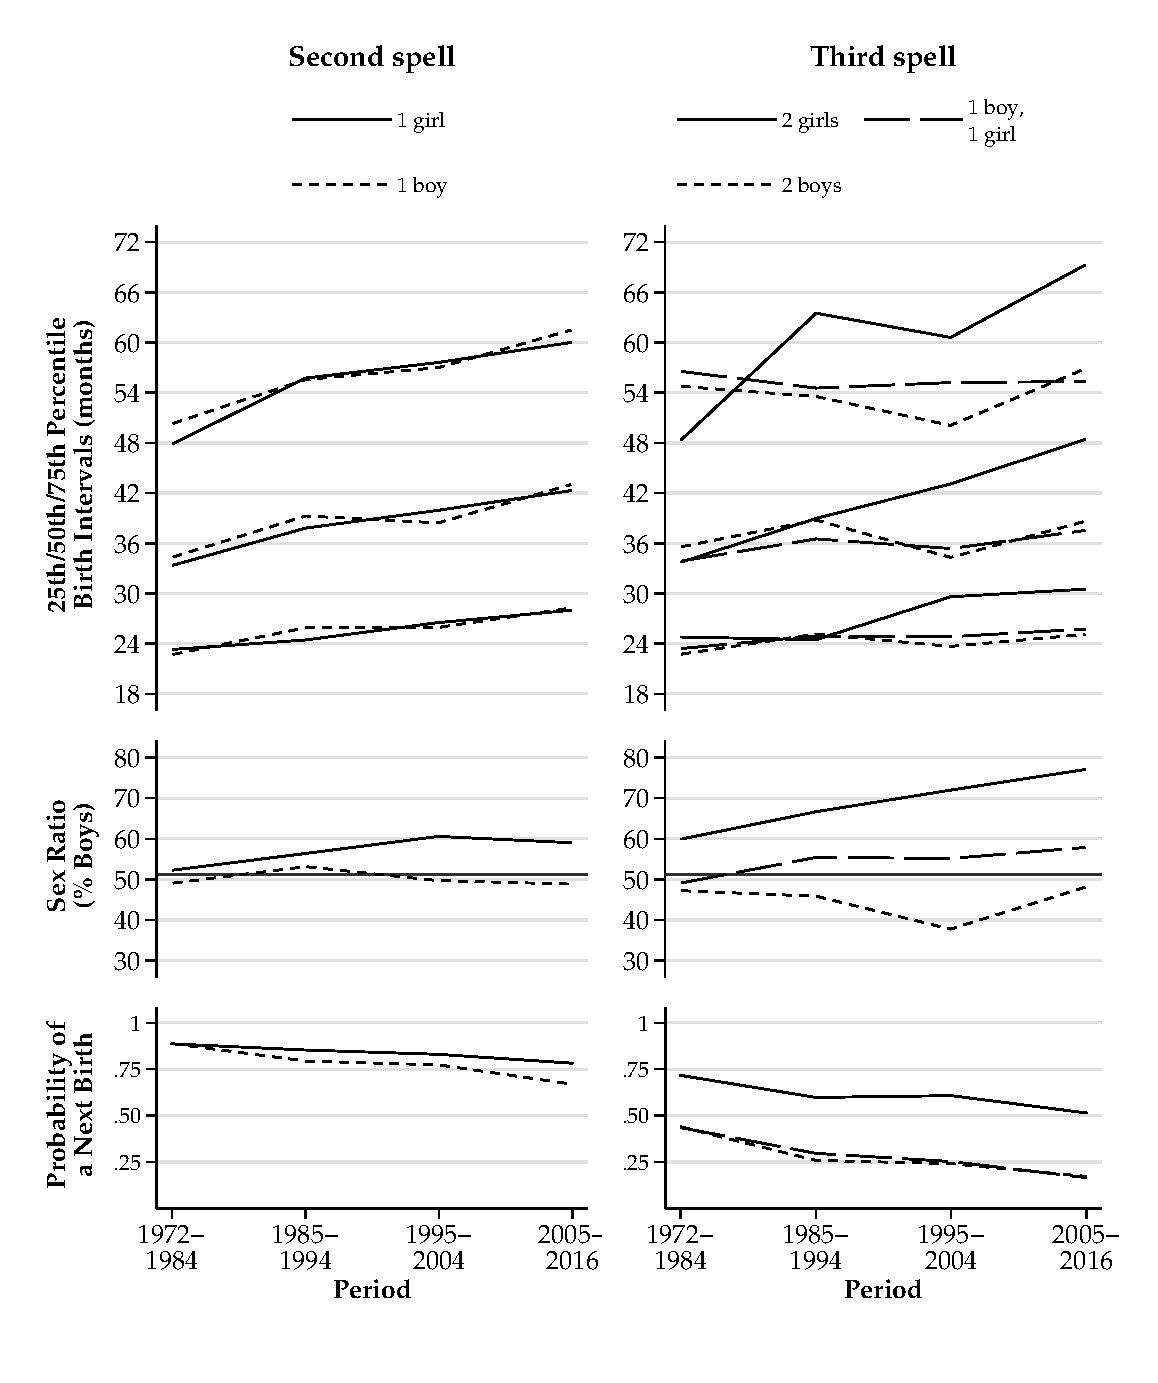
\includegraphics[width=\textwidth,height=\textheight,keepaspectratio=true]{bs_highest_urban}
% \caption{Percentile birth interval durations, sex ratios, and parity progression  
% for urban women with 12 or more years of education by spell, sex composition, and period}
% \label{fig:spacing_highest_urban}
\end{figure*}



\begin{figure*}
\centering
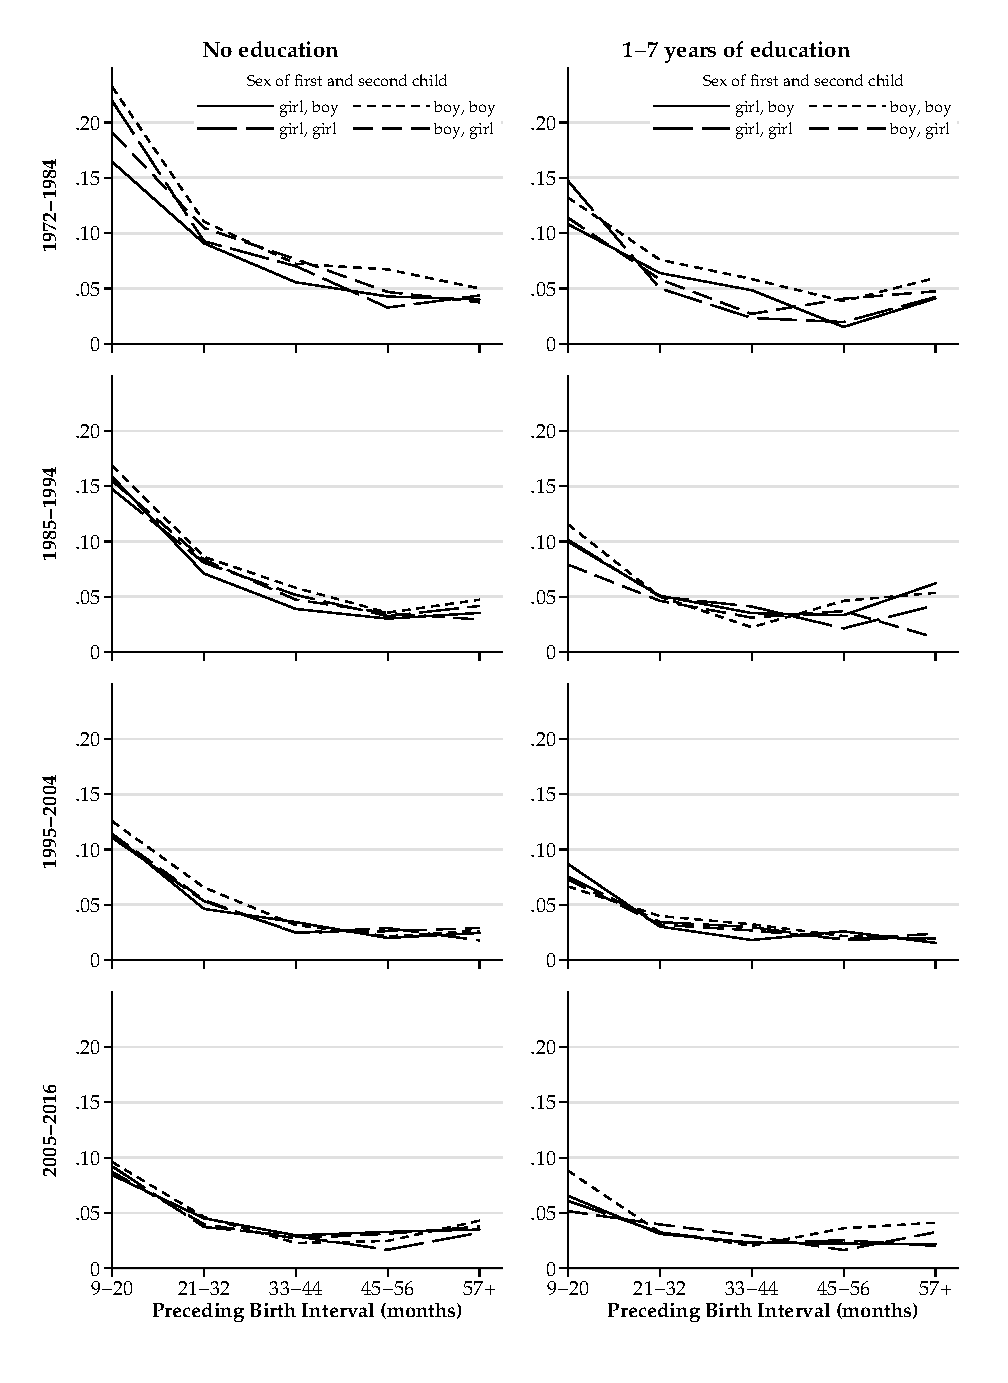
\includegraphics[width=\textwidth,height=\textheight,keepaspectratio=true]{mortality_spell_2_low_med}
% \caption{Infant mortality by preceding birth interval length across periods for second child of women with 
% no education and women with 1--7 years of education}
% \label{fig:mortality_low_med}
\end{figure*}


\begin{figure*}
\centering
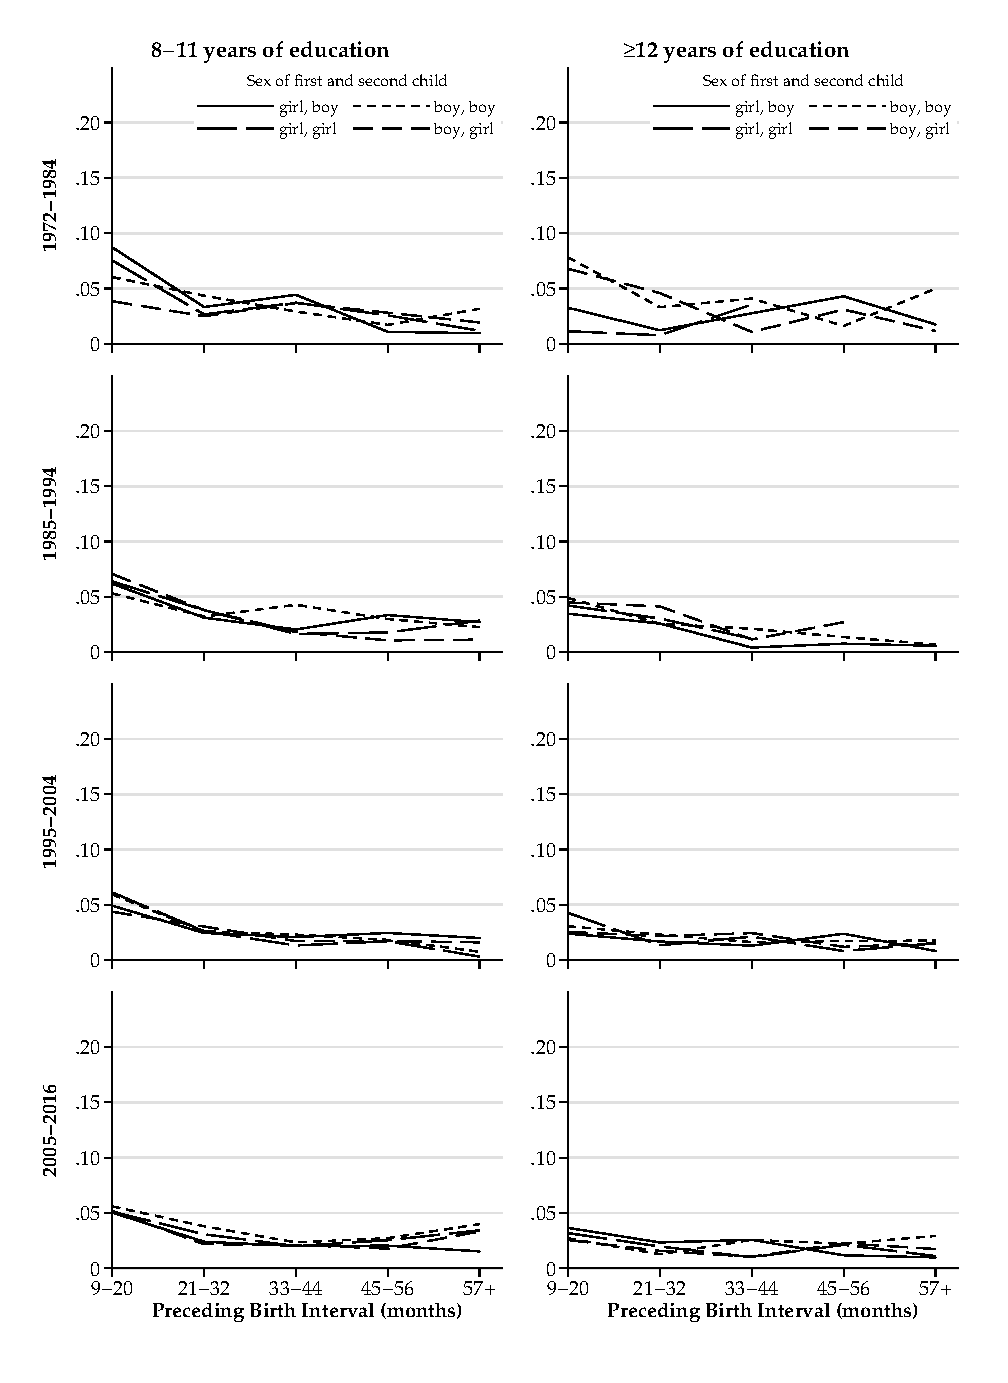
\includegraphics[width=\textwidth,height=\textheight,keepaspectratio=true]{mortality_spell_2_high_highest}
% \caption{Infant mortality by preceding birth interval length across periods for second child of women with 
% 8--11 and 12 and above years of education}
% \label{fig:mortality_high_highest}
\end{figure*}



\clearpage

\onehalfspacing
\bibliographystyle{aer}
\bibliography{sex_selection_spacing-final}

\addcontentsline{toc}{section}{References}


\end{document}



